%% main.tex — top-level file for the COLLIE paper (IEEE UV 2026).
%% Format: IEEE two-column conference template, 8th IEEE International
%% Conference on Universal Village (UV2026), October 17-20, 2026.
%% Regular papers: 5-8 pages; short papers: 3-4 pages; US Letter.
%%
%% Structure:
%%   sections/     one numbered .tex file per section, input below in order
%%   citations.bib the paper's bibliography (\bibliography below)
%%   figures/      all included graphics and TikZ/pgfplots figure sources
%%   illustrate/   scripts that generate the raster/PDF figures in figures/
%% The venue's annotated sample is conference_paper_instructions.tex;
%% IEEEexample.bib holds ready-made BibTeX entry patterns for every type.
%%
%% THIS IS AN INITIAL DRAFT. Experiments are still running. Every result cell,
%% every arm score, and every contrast is marked with \pending{...} and is
%% listed in the placeholder inventory in README.md. Every substantive claim is
%% traced to its evidence in CLAIMS.md. Run `make check` for the structural
%% checks; the placeholder total it prints must match the inventory table.

\documentclass[conference]{IEEEtran}
\IEEEoverridecommandlockouts
% The preceding line is only needed to identify funding in the first footnote. If that is unneeded, please comment it out.

%%% --- Required by IEEEtran ---------------------------------------------------
\usepackage{cite}

%%% --- Encoding ----------------------------------------------------------------
\usepackage[T1]{fontenc}
\usepackage[utf8]{inputenc}

%%% --- Math --------------------------------------------------------------------
\usepackage{amsmath,amssymb,amsfonts}
\usepackage{bm}
\usepackage{algorithmic}
% IEEEtran already defines \proof / \endproof, so amsthm must be told to take
% them over rather than error on a redefinition.
\let\proof\relax
\let\endproof\relax
\usepackage{amsthm}
\newtheorem{theorem}{Theorem}
\newtheorem{lemma}{Lemma}

%%% --- Graphics ----------------------------------------------------------------
\usepackage{graphicx}
\graphicspath{{figures/}}   % all figures live in figures/
\usepackage{xcolor}
\usepackage{tikz}
\usetikzlibrary{arrows.meta,positioning,fit,calc,backgrounds,decorations.pathreplacing}
\usepackage{pgfplots}
\pgfplotsset{compat=1.18}

%%% --- Tables --------------------------------------------------------------------
\usepackage{booktabs}
\usepackage{array}
\usepackage{multirow}
\usepackage{tabularx}
\usepackage{siunitx}
\newcolumntype{Y}{>{\centering\arraybackslash}X}   % centered tabularx column

%%% --- Captions -----------------------------------------------------------------
\usepackage{caption}
\captionsetup[table]{font={footnotesize,sc},labelsep=period}
\captionsetup[figure]{font={footnotesize},name={Fig.},labelsep=period}

%%% --- Header / footer ------------------------------------------------------------
% DISABLED to comply with the UV2026 call, which asks submissions to carry no
% running headers or footers and no page numbering. IEEEtran's conference mode
% already omits headers and page numbers on its own, so nothing replaces this.
% Kept, with the copyright block further down, for camera-ready: re-enable both
% together if the venue asks for the ISBN footer. See README.md, section 1.
% \usepackage{fancyhdr}
% \renewcommand{\headrulewidth}{0pt}
% \renewcommand{\footrulewidth}{0pt}

%%% --- Miscellaneous --------------------------------------------------------------
\usepackage{textcomp}
\usepackage{comment}
\usepackage{url}          % line-breakable URLs via \url{}
% [hidelinks] because the UV2026 call asks for no blue underlining on URLs and
% email addresses.
\usepackage[hidelinks]{hyperref}

%%% --- IEEE customizations ----------------------------------------------------------
\renewcommand\IEEEkeywordsname{Keywords}   % rename 'Index Terms' -> 'Keywords'

%%% --- The placeholder convention ---------------------------------------------------
% Every number, figure datapoint, and result sentence that the experiments have
% not yet produced is wrapped in \pending. The convention is mandatory: a
% half-filled draft must be impossible to mistake for a finished one. Grep
% "pending" over the tree and the count must match the inventory table in
% README.md exactly.
%
% \pending is a TEXT command. It must never appear inside a math environment.
\newcommand{\pending}[1]{\textcolor{red}{\textbf{[PENDING: #1]}}}
% Table cells that will receive a single scalar. Same convention, shorter.
\newcommand{\pcell}{\textcolor{red}{\textbf{PENDING}}}

%%% --- Notation shorthands ----------------------------------------------------------
\newcommand{\Filt}{\mathcal{F}}
\newcommand{\Ind}{\mathbb{1}}
\newcommand{\Real}{\mathbb{R}}
\newcommand{\Prob}{\mathbb{P}}
\newcommand{\Expect}{\mathbb{E}}
\newcommand{\shockspec}{\textsc{ShockSpec}}
\newcommand{\controlconfig}{\textsc{ControlConfig}}
\newcommand{\alertspec}{\textsc{AlertSpec}}
\newcommand{\eprocess}{e\nobreakdash-process}
\newcommand{\evalue}{e\nobreakdash-value}
\newcommand{\collie}{\textsc{Collie}}
\newcommand{\evalpath}{\texttt{eval/}}
\newcommand{\envpath}{\texttt{env.py}}

%%% --- Author block commands --------------------------------------------------------
\makeatletter

% \linebreakand: ends the current author row and starts a new one
% See https://tex.stackexchange.com/questions/509433/how-to-line-up-author-names-in-ieee-template
\newcommand{\linebreakand}{%
  \end{@IEEEauthorhalign}
  \hfill\mbox{}\par
  \mbox{}\hfill\begin{@IEEEauthorhalign}
}

% \AuthorCell[width]{name}{affiliation}
% Fixed-width name+affiliation cell, centered. Optional width defaults to 0.33\textwidth (3-col rows).
% Use \AuthorCell[0.45\textwidth]{...}{...} for 2-col rows.
\newcommand{\AuthorCell}[3][0.33\textwidth]{%
  \IEEEauthorblockN{\parbox[t]{#1}{\centering #2}}%
  \IEEEauthorblockA{\parbox[t]{#1}{\centering #3}}%
}

% \CorrespondingMark[n]: footnote + superscript for corresponding author (default ref 1)
\newcommand{\CorrespondingMark}[1][1]{%
  \thanks{\IEEEauthorrefmark{#1}Corresponding author}\IEEEauthorrefmark{#1}%
}

\makeatother

\begin{document}

% No manual line breaks: IEEEtran centres and wraps a title better than a
% hand-chosen break, which rewrapped badly at this length.
\title{Ask What Changed, Not What to Order: Typed Shock Hypotheses,
Compiled into an Inventory Controller, Activated by an Anytime-Valid
\eprocess{}}

% AUTHOR LINE, non-anonymous. Review is NOT blind: the IEEE UV 2026 call for
% papers (verified 2026-09-17, URL and quote in README.md) contains no mention
% of blind or anonymous review, the venue's own annotated sample ships a full
% \author block with affiliations and emails, and the submission instructions
% distribute no anonymous style file. The names themselves are \pending{}
% because the author list is the submitting authors' to set.
\author{
\AuthorCell{\pending{author list}\CorrespondingMark}{%
  \pending{affiliation} \\
  \pending{email}}

% Add co-authors as additional cells; \and separates cells within a row and
% \linebreakand starts a new row. Delete \CorrespondingMark above if unneeded.
% \and
% \AuthorCell{Given Name Surname}{%
%   \textit{dept. name of organization (of Aff.)} \\
%   \textit{name of organization (of Aff.)}\\
%   City, Country \\
%   email address or ORCID}
}

\maketitle

%%% --- Copyright and conference header / footer ----------------------------------
% DISABLED for submission. The UV2026 call asks submissions to carry no running
% headers or footers and no page numbering, and the call governs. The venue's
% own annotated sample installs the page-1 copyright footer below, which is
% required at camera-ready, so the block is kept verbatim rather than deleted.
%
% To re-enable at camera-ready: uncomment this block AND the fancyhdr lines in
% the preamble, then set the session designation, which is a placeholder.
% \thispagestyle{fancy}
% \fancyhead{}
% \fancyfoot{}
% \lhead{IEEE 8th International Conference on Universal Village · UV2026 · Session XX-X}
% \lfoot{\fontsize{8}{10} \selectfont 979-8-3195-2714-1/26/\$31.00 \copyright2026 IEEE}
% \rhead{}
% \cfoot{}
% \rfoot{}

%%% --- Sections (one file per section, in paper order) -----------------------------
% sections/00_abstract.tex -- abstract and keywords.
% IEEE UV 2026: the abstract submitted through EasyChair is 100-300 words, with no symbols,
% special characters, footnotes or math; this one follows the same rule.

\begin{abstract}
Language models can read the operational messages that precede supply and demand shocks,
but acting on what they say is risky: a wrong reading moves real orders. We study a
replenishment controller that asks a language model only what changed, in a closed typed
vocabulary, and tests the answer with an anytime-valid e-process on data that arrive after
the proposal. A preregistered pilot of the natural design, which lets a hypothesis act only
once its e-process crosses a Ville threshold, was stopped at its own decision gate: the
gate was safe but acted late, rarely, and on magnitudes the model got wrong. We therefore
propose certify-then-hedge. The e-process no longer switches the controller on; it prices
a fixed set of action-aligned hypotheses, the model's answer only sets prior weights over
them, the size of the shock is estimated from the data, and the order is the critical
fractile of the resulting posterior-predictive mixture. The expected exposure to a false
hypothesis stays below the frozen error budget at every stopping time, whatever the model
says, and the old gate is the special case of acting on the most probable hypothesis. On
240 fresh episodes registered before any outcome was seen, certify-then-hedge improved net
reward over the gate by 309 and 179 per episode and over the operations research baseline
by 179 and 163, with Gemini and Grok as the proposers, all four tests surviving Holm
correction, and it was non-inferior on no-shock episodes. Four further models, from an
eight-billion-parameter open model to a legacy chat model, gave the same picture, while
acting on proposals at once lost 1,478 to 3,181 per episode. On this simulator the gain comes
from the statistics rather than the language: a content-free variant earns as much, and the
model's contribution is to cut commitment on no-shock episodes by about 45 percent.
\end{abstract}

\hfill

\begin{IEEEkeywords}
large language models, inventory control, anytime-valid inference, e-values, sequential
decision making, preregistration
\end{IEEEkeywords}
          % abstract and keywords
\section{Introduction}

\begin{figure*}[!t]
\centering
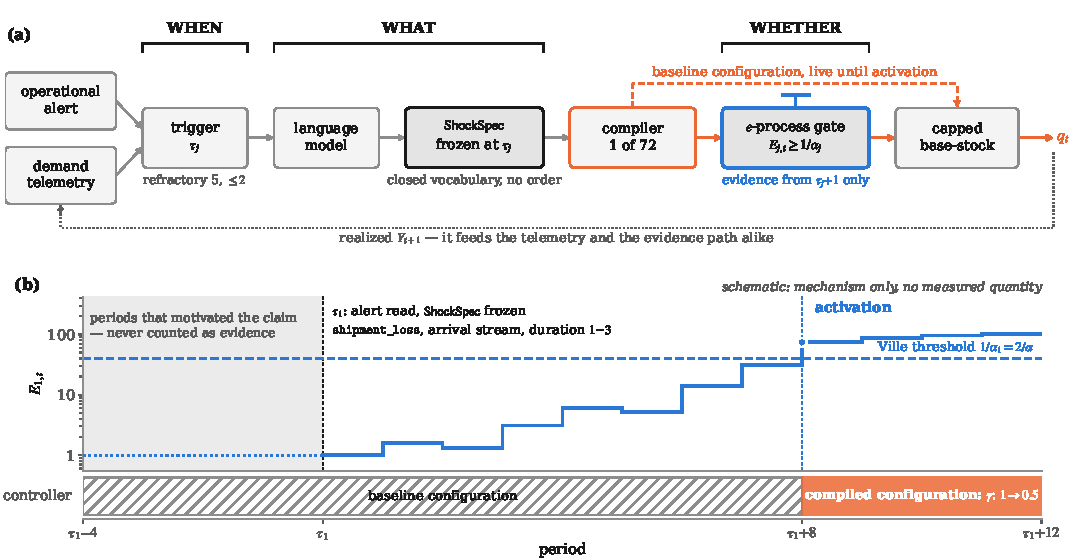
\includegraphics[width=\textwidth]{fig1_overview.pdf}
\caption{The registered gate and certify-then-hedge on the same input, one fresh-seed episode
chosen post hoc to show the mechanism: of the 32 lead-time episodes, it is the gate's third-worst
and the hedge's tenth-lowest. \textbf{(a)}~At period~13 the alert yields a \shockspec{} from
Gemini~3.8 Flash (six of its nine fields shown) naming a lead-time shift of \emph{medium}
magnitude; the true shift is one period, from period~14. \textbf{(b)}~The gate tests the stated
hypothesis alone and, once $E_{j,t} \ge 1/\alpha_j$, from period~24 (eleven periods after the
alert) switches all at once to the configuration compiled from the stated magnitude, two extra
periods. \textbf{(c)}~Certify-then-hedge keeps the fixed set $\mathcal{H}$, which the answer only
reweights (prior $a_j w_{jk}$, with $a_j$ the firing's share of the error budget $A$), prices each
hypothesis by its own \protect\eprocess{}, estimates a one-period shift from the data (from
period~18, by replay of the frozen arm) and orders the $p/(p+h)$ quantile of the
posterior-predictive mixture. Its bound needs a known null and arrival law; as run, a null
simulation puts $\Expect_0[\Pi_\sigma]$ at up to $2.7A$ (Section~\ref{sec:limitations}). Each lane
ends in the episode from period~10 (every series is zero before it): commitment and cumulative
net reward against arm~1. Over all 32 lead-time episodes the hedge gains $+1{,}286$ per episode
on arm~1 (registered readout) and the gate, post hoc, $+414$.}
\label{fig:overview}
\end{figure*}

Language models are being proposed for replenishment decisions. On InventoryBench, 1{,}320 multi-period
lost-sales replenishment instances, the strongest published language-model strategy lets the
model name an order quantity every period and applies it untested~\cite{inventorybench}.
Whether that works cannot be read off the reported gain, because three decisions are welded
together: \emph{when} the model is consulted, \emph{what} it may say, and \emph{whether} its
answer is trusted. Reproducing the benchmark's operations research baseline also showed that
its published score belongs to a legacy simulator (Section~\ref{sec:background}), so the
evidence is partly artifactual as well as bundled.

We took the three decisions apart. A shared trigger decides when the model is asked; a closed
schema, the \shockspec{}, fixes what it may say (a typed claim about what changed in the
exogenous process, never an order); and an anytime-valid \eprocess{}, started strictly after
the proposal, decides whether the claim may touch an order. We preregistered the natural
version of the last step, a \emph{gate} that lets a hypothesis act only once its \eprocess{}
crosses the Ville threshold $1/\alpha_j$, and ran a pilot against a frozen decision rule.

The gate failed its own decision rule: the registered pilot read \emph{kill-or-reframe}, and
an exploratory rerun with live Gemini and Grok answers showed why. The gate rarely acted on a
false alarm (1 of 12 false-alert episodes with each model), but it acted on fewer than half of
the right-family proposals (43\% and 39\%), a median of 10 and 11 periods after they were made,
and then compiled whatever magnitude the model had stated, though no alert states a size
(Section~\ref{sec:results}).

This paper replaces the gate with \emph{certify-then-hedge}. The \eprocess{} no longer switches
the controller on; it prices a fixed set of action-aligned hypotheses. The language model's
answer only reweights that set (and fixes the onset window of the hypothesis it names), mixed
with a uniform prior so that a wrong answer has bounded cost. The size of a shock is estimated
from the data rather than taken from the model, and the order is the critical fractile of the
posterior-predictive mixture, so the controller moves toward a hypothesis as fast as the
evidence for it grows (Fig.~\ref{fig:overview}). Under a known null and arrival law, the construction keeps the
gate's error budget as a bound on expected exposure to a false hypothesis at every stopping
time, whatever the model says, and in the single-hypothesis case the gate's threshold is
analogous to a posterior-odds rule.


\subsection*{Contributions}

\begin{itemize}\itemsep0pt
\item \textbf{Certify-then-hedge}, a graded commitment rule for typed language-model
      hypotheses in a closed control loop, with an exposure bound that holds for any model
      output under a known null and arrival law, an odds-regret bound in cost units, and a
      simulation of how far the bound slips under the null we ran (Section~\ref{sec:hedge}).
\item \textbf{Two registered tests on fresh seeds}, exploratory with respect to the project's
      preregistration. At the middle cost ratio, against the gate and against the operations
      research baseline, with two proposer models, all four primary tests survive Holm
      correction and losses on no-shock episodes stay within the registered margin. At the
      benchmark's other two ratios the gains over the gate hold; at the higher one so does the
      gain over the baseline, and the model's answer adds value with one of the two models, but
      non-inferiority on no-shock episodes is not established there; on noisy lead times the
      gain over the baseline is not confirmed (Section~\ref{sec:results}).
\item \textbf{An account of where the gain comes from.} Against the baseline it comes almost
      entirely from lead-time shifts, and an alert-timed variant that ignores the model's
      answer is not distinguishable from it with the two primary models;
      the model's label lowers commitment on no-shock episodes and, post hoc, shows no
      detectable change in their reward. A model ladder (20 of 21 models run) shows, post hoc, that acting on proposals at once
      loses more the more readily a model commits, and that being right does not protect it.
\item \textbf{The negative pilot and the audit trail}: the gate's registered failure, every
      deviation and disclosure, and the audited benchmark divergence that motivated the
      controlled design.
\end{itemize}

\section{Testbed}
\label{sec:background}

\textbf{The audited benchmark.} InventoryBench~\cite{inventorybench} has 1{,}320 lost-sales
instances (720 synthetic, 600 from weekly apparel sales). Each period the policy orders, then
receives, then sells, then pays holding on ending stock; demand is observed uncensored, and
in-transit stock is a single scalar with no shipment ages. Every cell is an integer, so our
reimplementation is checked for exact equality rather than a tolerance: it matches the official
pipeline with a maximum absolute difference of $0.0$ over 648 comparisons, and our arm~1
reproduces all 1{,}320 published baseline order sequences bit for bit. That reproduction
exposed a \emph{harness divergence}\label{sec:divergence}: the benchmark's legacy simulator keeps
a lost shipment in in-transit stock forever, while its submission path never adds it. The
published baseline score of $0.4447$ belongs to the legacy simulator; under the authoritative
submission path the same policy scores $0.5208$, and the difference is exactly the 440
instances that contain a lost shipment.

\textbf{Shock episodes.} To study hypotheses whose truth is known, we generate episodes on the
same event order: stationary demand (mean 100, standard deviation 25) plus one of six shock
families, a demand-level shift up or down, a temporary demand pulse, a lead-time shift, a
shipment-loss burst, and a compound demand-and-pause shock, with the onset drawn in periods
14 to 22 of 50. Each unit is replayed under four information conditions: no alert, an accurate
alert one period before onset, the same alert two periods after onset, and an unreliable alert
(overstated, ambiguous or a distractor), drawn from a bank of team-written templates; each
unit also has an unshocked twin that serves as a null episode, silent or with a false alert.
Profit is 4 and holding 1 per unit, so the critical fractile is $0.8$. The reward we report is
\emph{net}, profit minus holding, which is the benchmark's own score; gross profit, the
endpoint of our first registration, charges no holding and is reported alongside.

\section{Problem Setup}
\label{sec:setup}

What must the information structure respect for a sequential test to be
legitimate inside a closed control loop?

Let $I_t$ be on-hand inventory at the start of period $t$, $P_t$ the aggregate
in-transit total, $A_t$ our order, $R_t$ aggregate receipts, and $p$ and $h$ the
per-unit profit and holding cost. The order is coerced by the benchmark's truncation
and capped as $A_t = \min(\max(0, \lfloor q_t \rfloor), C_t)$ (every controller
here already returns an integer) and dispatched with a latent transit time, and our
endpoints accumulate net reward and gross profit under the audited event order. Let $Y_t$ be the exposed observable,
uncensored demand in the headline setting, and $\Filt_t$ the sigma-algebra
generated by everything observed \emph{before} $A_{t+1}$ is chosen, $Y_t$
included. Two properties follow. \textbf{(A1) Actions are
predictable:} $A_t$ is $\Filt_{t-1}$-measurable, and the runner builds and freezes
the observation before calling the controller, so this holds by construction
rather than by convention. \textbf{(A2) Actions affect only the future:} $A_t$
influences $Y_{t+1}$ and later, never $Y_t$. Conditioning $Y_r$ on
$(\Filt_{r-1}, A_{r-1})$ is therefore well defined and does not condition on
anything $A_{r-1}$ could have altered retroactively, and every density below is
written that way. A zero actual lead time moves $R_t$ rather than $Y_t$, so (A2)
survives. Finally, $\tau_j$ is the proposal period of hypothesis $j$ and a
stopping time, $h_j$ the \shockspec{} frozen there, and $E_{j,t}$ its evidence
process.

\section{\shockspec{}: The Typed Commitment}
\label{sec:spec}

\begin{figure*}[!t]
\centering
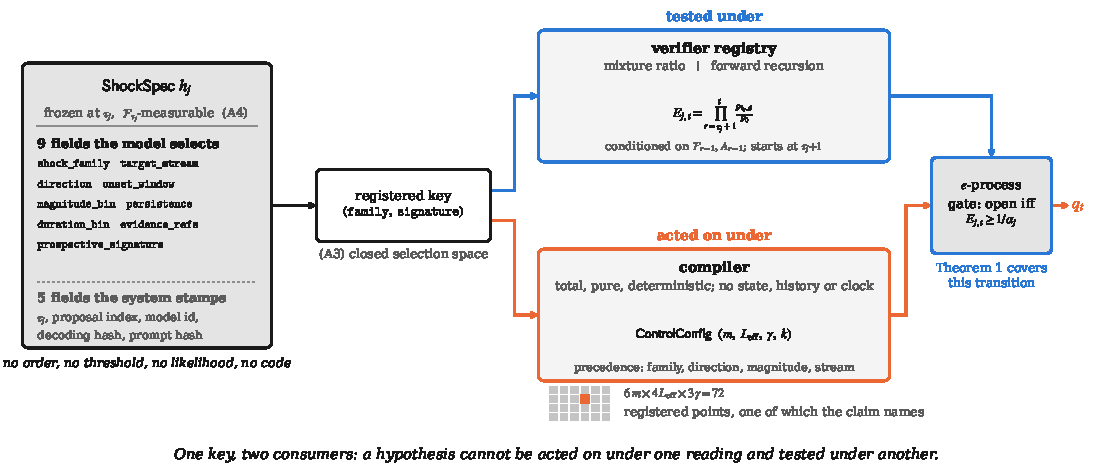
\includegraphics[width=\textwidth]{fig2_method.pdf}
\caption{One key, two consumers. The typed hypothesis leaves the model once and
is then read twice, by two machines that must not be allowed to disagree.
Downward, the compiler of Section~\ref{sec:compile} turns it into one point of
the registered 72-point grid, and the controller acts on that point. Upward, the
registry of Section~\ref{sec:verify} resolves the \emph{same} key into the
verifier construction that will test it. Both branches hang off one key, which
is the property that matters: a hypothesis cannot be acted on under one reading
and tested under another. The two branches meet again at the gate, and only the
transition it governs is covered by Theorem~\ref{thm:activation}.}
\label{fig:method}
\end{figure*}

What is the model allowed to say? Exactly one object, drawn from a vocabulary the
system froze before any test episode ran. Closing that vocabulary is what makes
the later test admissible rather than decorative.

At the proposal period $\tau_j$ the model receives only information in
$\Filt_{\tau_j}$: the permitted product text, any alert visible then, the demand
and arrival history, the inventory position, an aged pipeline summary and the
costs. It must return valid JSON under a closed schema that
forbids unknown keys and yields an immutable object. The model selects nine
fields. \texttt{shock\_family} is one of \texttt{no\_change},
\texttt{demand\_level}, \texttt{temporary\_pulse}, \texttt{lead\_time\_shift},
\texttt{shipment\_loss}, \texttt{transit\_pause} or \texttt{compound}.
\texttt{target\_stream} ranges over demand, arrival, both and none, and
\texttt{direction} over the six registered directions. \texttt{onset\_window} is
a registered offset pair or null, while \texttt{magnitude\_bin},
\texttt{persistence} and \texttt{duration\_bin} take their registered bins.
\texttt{evidence\_refs} points at visible message spans or observation
identifiers, and \texttt{prospective\_signature} is schema-defined. Five fields
are stamped by the system and never by the model:
$\tau_j$, the one-based proposal index, the model identifier, the decoding hash
and the prompt hash. \texttt{no\_change} is a first-class output rather than a
failure code, and an accepted abstention is scored separately from a formatting
failure because capability and reliability should not share a cell.
\texttt{transit\_pause} is a first-class family even though no generator family
emits it alone, since it is the supply leg of family 6.

The model selects a key. It cannot write a falsifier, a likelihood, a threshold,
an order equation, or code: the system maps the pair (\texttt{shock\_family},
\texttt{prospective\_signature}) to a verifier construction and the whole object
to controller parameters. Fig.~\ref{fig:method} draws that split, and drawing
both arrows off one key is the whole content of the figure. An invalid object gets one format-repair attempt, a
second failure falls back to the unchanged baseline, and every attempt is counted
as accepted, accepted after repair, or fallback. The restriction is load-bearing:
if the model could invent its own vague test after seeing the trigger window,
falsifiability would be cosmetic. Two structural facts remove the
circularity. \textbf{(A3) Closed selection space:} the hypothesis is drawn from a
registered vocabulary whose map to a construction is frozen. \textbf{(A4) Frozen
at a stopping time:} $\tau_j$ is a stopping time, $h_j$ is
$\Filt_{\tau_j}$-measurable, and its evidence product starts at $\tau_j + 1$. For
the carrier suspension the model is expected to return \texttt{shipment\_loss} on
the \texttt{arrival} stream, direction \texttt{arrival\_interrupted}, duration bin
\texttt{1\_3}, with \texttt{evidence\_refs} naming the alert and the arrival
residual. Nothing in that object is an order. It says what changed.

\section{Compilation: From a Claim to an Order}
\label{sec:compile}

How does a sentence about the world become an order quantity? Through a total,
pure, deterministic function with no episode state, history or clock.

A \controlconfig{} is a four-tuple $(m, L_{\mathrm{eff}}, \gamma, k)$ with
$m \in \{0.6, 0.75, 1.0, 1.25, 1.5, 2.0\}$, $L_{\mathrm{eff}} \in \{1,2,3,4\}$
and $\gamma \in \{0, 0.5, 1\}$, which is $6 \times 4 \times 3 = 72$
configurations. The fourth entry is a pure function of the other three, obtained
by comparing the point against the grid reference on two flags, whether the
compiled belief moves demand and whether and how it moves the supply side. That
key has two consumers: control acts on it, and Section~\ref{sec:verify}'s
registry resolves the same key into the construction that will test it, so a
hypothesis cannot be acted on under one reading and tested under another. Note
that $L_{\mathrm{eff}}$ is a compiled \emph{belief} and never the observation's
promised lead time, because the compiler is a pure function of the \shockspec{}
alone. Precedence is fixed as family, then direction, then magnitude bin, then
target stream.

\begin{table}[!tb]
\caption{The registered compiler table, by severity rank, as absolute points
around the grid reference $(1, 1, 1)$.}
\label{tab:mapping}
\centering
\footnotesize
\begin{tabular}{@{}llll@{}}
\toprule
Shape & $m$ & $L_{\mathrm{eff}}$ & $\gamma$ \\
\midrule
\texttt{demand\_level} up      & 1.25 / 1.5 / 2.0 & 1 & 1.0 \\
\texttt{demand\_level} down    & 0.75 / 0.6 / 0.6 & 1 & 1.0 \\
\texttt{temporary\_pulse} up   & 1.25 / 1.5 / 2.0 & 1 & 1.0 \\
\texttt{temporary\_pulse} down & 0.75 / 0.6 / 0.6 & 1 & 1.0 \\
\texttt{lead\_time\_shift}     & 1.0 & 2 / 3 / 4 & 1.0 \\
\texttt{shipment\_loss}        & 1.0 & 1 & 0.5 / 0.0 / 0.0 \\
\texttt{transit\_pause}        & 1.0 & 2 / 2 / 3 & 1.0 / 1.0 / 0.5 \\
\texttt{compound}              & 1.25 / 1.25 / 1.5 & 2 / 2 / 3 & 1.0 \\
\texttt{no\_change}            & 1.0 & reference & 1.0 \\
\bottomrule
\end{tabular}
\end{table}

A lead-time shift moves $L_{\mathrm{eff}}$ alone, because arrivals are still
coming, while a shipment loss moves $\gamma$ alone, because arrivals keep their
timing but fewer can be trusted to be real. A pause is deliberately asymmetric,
since under the authoritative harness nothing inflates the pipeline count for
$\gamma$ to correct. Composition is reference-relative, because an absolute grid
point applied wholesale would move axes the hypothesis does not concern, and a
demand-up hypothesis compiled to $L_{\mathrm{eff}} = 1$ against a promised lead
time of 2 cancels its own demand signal exactly. An axis left at the reference is
inherited, and a moved axis applies absolutely for $m$, as an offset for
$L_{\mathrm{eff}}$ and as a ratio for $\gamma$.

One controller serves every arm that routes through the compiler, differing only
in which configuration is active in a period. With $\bar{d}_t$ and $s_{d,t}$ the
running mean and sample standard deviation of the training samples followed by
every demand observed so far, and $z^\star = \Phi^{-1}(p/(p+h))$ the
newsvendor critical fractile~\cite{arrow-harris-marschak, zipkin-foundations},
\begin{align}
IP_t &= I_t + \gamma P_t, \\
S_t  &= m\,(1 + L_{\mathrm{eff}})\,\bar{d}_t
        + z^\star \sqrt{1 + L_{\mathrm{eff}}}\; s_{d,t}, \\
q_t  &= \min\bigl(\max(0, \lceil S_t - IP_t \rceil),\; C_t,\; \hat{C}_t\bigr).
\end{align}
The critical fractile is read from the per-period cost columns rather than
assumed constant, putting $z^\star$ at the $0.95$, $0.80$ and $0.50$ quantiles
across the three registered cost ratios, and $\hat{C}_t$ is the published
baseline's own internal smoother, kept separate from our cap $C_t$ because they
are different objects that share a word. The property that makes the ladder
legitimate is that at the per-instance baseline configuration this controller
reproduces arm~1 bit for bit, so ``the published operations research policy is
running'' is literally true for every arm while no hypothesis is active. For the
running example the compiled point is $\gamma = 0.5$ at low severity and
$\gamma = 0$ above it, so the inventory position shrinks by the discounted
pipeline and the controller replaces the shipments it no longer believes in. That
is the whole intervention.

\section{Certification: The E-Process and the Gate}
\label{sec:verify}
\label{sec:notclaim}

For a proposal $j$ with registered null $p_0$ and alternative region $\Theta_j$,
\begin{equation}
E_{j,t} \;=\; \int_{\Theta_j}
\prod_{r=\tau_j+1}^{t}
\frac{p_{h_j,\theta}\bigl(Y_r \mid \Filt_{r-1}, A_{r-1}\bigr)}
     {p_0\bigl(Y_r \mid \Filt_{r-1}, A_{r-1}\bigr)}
\; dW_j(\theta),
\label{eq:eprocess}
\end{equation}
with $E_{j,\tau_j} = 1$. Each fixed-$\theta$ ratio has conditional mean one under the null whatever policy generated
$A_{r-1}$, so the product is a test martingale even inside the closed loop, and a mixture over
$\theta$ with a prior $W_j$ fixed at $\tau_j$ is again one~\cite{ramdas-savi, e-detectors,
grunwald-safe-testing}. With $W_j$ discrete, the mixture sits outside the product. Demand
hypotheses use the exact law of rounded normal demand under a registered grid of multipliers,
starts and durations; arrival hypotheses use an exact forward recursion over the remaining
transit times of outstanding orders, so the verifier never uses the controller's imputed
shipment ledger; compound hypotheses split their budget over two separate
\eprocess{}es.

\textbf{The registered gate.} Arm~10 allocates $\alpha_j = \alpha 2^{-j}$ to proposal $j$ (at
most two per episode, $\alpha = 0.05$) and lets proposal $j$ act, on its compiled configuration,
from the first $t$ with $E_{j,t} \ge 1/\alpha_j$.

\begin{theorem}
\label{thm:activation}
Under the registered global no-change null, $\Prob_0(\text{any false activation in an
episode}) \le \sum_j \alpha_j \le \alpha$.
\end{theorem}

Ville's inequality~\cite{ville} bounds each crossing by $\alpha_j$ and a union bound gives the
rest. The guarantee is \emph{model-conditional}: it presumes $p_0$ is the true law. Two
implementation facts weaken it in ways we measured rather than assumed. The demand null's mean
and variance are estimated from the pre-proposal prefix, which makes the test anti-conservative
for short prefixes; and the registered arrival null is a diffuse lead-time law while our
generator's lead times are deterministic, which makes the arrival test slow but, empirically,
conservative. Neither theorem in this paper covers wrong-family activation, realized profit, or
refutation and expiry rules, which are registered operational rules rather than certified ones.

\section{Triggers and the Alert Bank}
\label{sec:triggers}

Who decides when the model is consulted, and where does the text come from? Both
are infrastructure rather than contribution, and we say so, because
event-triggered invocation is already well covered~\cite{event-triggered-llm}.
What matters is that the infrastructure be shared exactly enough that no
comparison can be confounded by it.

A proposal opportunity opens when an operational alert arrives or when a
calibrated telemetry detector crosses its threshold. Six rules exist: alert only,
CUSUM~\cite{page-cusum}, Page-Hinkley~\cite{hinkley-cusum-1971}, their disjunction with the alert channel,
which is the primary rule, and two budget-matched schedules. Detectors are
stateless about suppression: one emits a raw candidate and two wrappers decide,
composed as \texttt{MaxProposals(Refractory(}\textit{d}\texttt{, 5), 2)}, so the
window and the cap are uniform across rules, including rules written after the
design was frozen. Thresholds come from Monte Carlo on development and
calibration nulls only, at the nearest-rank 95th percentile of the per-episode
maximum statistic over 60 stationary twin paths, so three of 60 null episodes
fire by construction. The window of 5 periods covers the longest registered pulse
and pause, and the cap of 2 is the value $\alpha_j = \alpha\,2^{-j}$ was designed
around. Two properties matter for the claims. The demand-side detectors read only the
previous demand and the alert channel, both exogenous to the policy, so a trigger
trace is a pure function of the episode's demand and alert streams and two arms
sharing a rule must produce bitwise-identical traces, which the suite asserts.
Without that, a comparison between two arms would conflate a different invocation
pattern with a different policy. And a denylist, enforced at runtime on
every feature mapping and statically by a syntax-tree scan, forbids future demand
and arrivals, pattern names, instance identifiers, split and test labels and every
field of the hidden incident record. It is deliberately over-broad on substrings,
because a trigger that peeks is worse than a bad trigger: it looks like a good
one.

\textbf{What the detector cannot see.} Measured over 120 seeds per family at the
frozen calibration under the no-alert condition, the firing rate is $0.99$ for a
demand increase, $1.00$ for a demand decrease, $0.69$ for the temporary pulse,
$0.03$ for the lead-time shift, $0.03$ for the lost-shipment burst and $0.77$ for
the compound event. The two supply-only families sit at the null rate \emph{by
construction}, since a demand-side detector cannot see a lead-time shift or a
lost shipment. This is not a tuning failure to be fixed: it is what makes the
alert channel the only early signal for our running example.

\textbf{The alert bank.} The text channel is 180 short synthetic operational
templates, 60 per split and 10 per family within each split, of which four per
family-split cell are accurate, two overstated, two ambiguous and two operational
distractors, with wording families held out across splits and controlled slots
instantiated per episode. Template identity stays on the analysis side, because
language-level uncertainty must treat the template as a sampling unit and not the
rendered string, and synthetic messages are preferred because timing and
information content are controllable: a message must not carry information that
could not have existed when it is delivered. Two independent raters score every
template on five criteria, and leakage is not negotiable by consensus, since one
below-threshold score from either rater removes it. \pending{inter-rater
agreement and templates pruned for leakage} Each message also carries a hidden
\alertspec{}, and feeding that straight to the compiler is the perfect-parsing
upper bound. Every trajectory is crossed with the identical exogenous realization
under four information conditions, and the four cells of one seed are
\emph{paired replays of one independent unit}.

\section{The Arm Ladder and Honest Accounting}
\label{sec:ladder}

What cheaper thing would have worked just as well? Every rung in
Table~\ref{tab:ladder} is one answer, stated as a reviewer would state it, and
the rung above it is what remains once the answer is removed. The same table
carries the headline result slots, so the objection and the number that answers
it sit on one line.

\begin{table*}[!t]
\caption{The ladder and the headline result slot in one place. Each rung names
the objection it answers, and its three cells are the pre-built slots the sweep
will fill: stratum-weighted estimates on the submission harness with seed-level
cluster-bootstrap intervals over the independent unit. The last three rows are
the six confirmatory tests, Holm-corrected~\cite{holm-multitest} as one family.}
\label{tab:ladder}
\centering
\scriptsize
\begin{tabular}{@{}r@{~}p{0.175\textwidth}p{0.235\textwidth}ccc@{}}
\toprule
\# & Arm & Objection it answers & Profit & Lost sales & Norm.\ reward \\
\midrule
1  & capped base-stock & the published baseline & \pcell & \pcell & \pcell \\
2  & telemetry-only adaptive & a changepoint detector would do this & \pcell & \pcell & \pcell \\
3  & every-period direct action & just let the model order & \pcell & \pcell & \pcell \\
4  & triggered direct action & the gain is from calling less often & \pcell & \pcell & \pcell \\
5  & every-period parameters & the gain is from the OR layer & \pcell & \pcell & \pcell \\
6  & sparse ephemeral parameters & the gain is from sparsity & \pcell & \pcell & \pcell \\
7  & persistent parameters, fixed expiry & the gain is from persistence & \pcell & \pcell & \pcell \\
8  & \shockspec{}, immediate & the gain is from typing the hypothesis & \pcell & \pcell & \pcell \\
9  & \shockspec{}, heuristic rollback & a heuristic guard would do & \pcell & \pcell & \pcell \\
10 & \shockspec{}, \eprocess{} & \textbf{the contribution} & \pcell & \pcell & \pcell \\
11 & every-period recommendation, then model & the strongest published method & \pcell & \pcell & \pcell \\
\midrule
   & CUSUM to compiler & does telemetry alone suffice & \pcell & \pcell & \pcell \\
   & keyword parser & does reading the message need a model & \pcell & \pcell & \pcell \\
   & \alertspec{} upper bound & ceiling for perfect parsing & \pcell & \pcell & \pcell \\
   & oracle headroom & ceiling the compiler can reach at all & \pcell & \pcell & \pcell \\
\midrule
   & C1, arm 10 vs arm 8 & does verification earn its place & \pcell & \pcell & \\
   & C2, arm 10 vs arm 6 & does typing beat ephemeral parameters & \pcell & \pcell & \\
   & C3, arm 10 vs arm 11 & does it beat the best published method & \pcell & \pcell & \\
\bottomrule
\end{tabular}
\end{table*}

Arms 3, 5 and 11 reproduce the benchmark's own three language-model
strategies~\cite{inventorybench} on a prompt builder asserted byte-identical to the published agent's prompt at the
same state, which is what makes arm 3 a fair representation of the existing
approach rather than a strawman. Arm 7's expiry equals the frozen refractory
window, so it measures persistence rather than a longer invocation budget, and
arms 4 and 6 are matched to arms 3 and 5 on \emph{realized} calls.
Arm 9's guard is real: an observation contradicts the spec when it lands more than
one baseline standard deviation on the wrong side of the pre-proposal baseline
mean for the spec's direction, and two consecutive contradictions refute it. Four
further arms route through the identical compiler and controller, so a difference
between any two is a difference in what reached it: a detector, a keyword parser,
the hidden \alertspec{} as the perfect-parsing ceiling, and an oracle
\shockspec{} as the headroom bound. Only the last two may read hidden truth.

Arms 8, 9 and 10 build the same proposal prompt at the same decision point and
differ only in the injected activation policy, and the cache collapses those to
one physical request with one charged copy per arm. Two tests carry the design:
one asserts that the physical call set is shared, the other asserts
\emph{divergence}, that identical proposals produce different activation traces.
If they did not, the activation stage would be doing nothing.

\textbf{Physical against charged.} Every cost claim depends on this. A
\emph{physical} entry is what the provider saw, one per real request, and a
\emph{charged} entry is what an arm would have paid, one per arm per call it would
have made, including calls served from cache. Arms 8, 9 and 10 sharing one
proposal call therefore produce one physical and three charged entries, and
$\text{physical} \le \sum_{\text{arms}} \text{charged}$ becomes a property of the
books, asserted over random arm sets. Every attempted call is classified exactly
once when the arm settles it, an unsettled charged entry fails a conservation
check, and dated cost is computed at log time from the registered price table. The configuration is cloud-only, with a hosted Gemini
Flash endpoint as the primary at \$0.75 per million input and \$3.75 per million
output tokens including thinking tokens, retrieved 2026-09-06~\cite{gemini-pricing}, and a different
provider for confirmation.

\section{Experimental Design}
\label{sec:experiments}

What would count as evidence, and what was decided before any test trajectory
ran? This section is design only. The experiments are running, so every cell is
marked \pending{like this} and every table is a pre-built slot.

\textbf{Splits, and the independent unit.} Seeds come from disjoint reserved
pools of 36 development units, 24 calibration units and 150 test units, six
families by six, four and twenty-five seeds. Each test unit is crossed with the
four information conditions, giving 600 paired replays plus 20 silent-null and 20
false-alert-null controls, so 640 held-out rollouts per sparse arm, with every
threshold and mapping frozen on development and calibration data. \textbf{The independent unit is the seed, not the rollout.} The four
information cells of one seed are paired replays of one exogenous trajectory, so
treating them as four samples would inflate the effective sample size fourfold
and narrow every interval by roughly half, invisibly. The evaluation engine is
therefore registered to refuse any confirmatory statistic computed from a frame
with more than one row per pair of independent unit and arm, and to raise rather
than warn. Family tail estimates stay exploratory even at twenty-five seeds, and
every language-level claim bootstraps jointly over seed and template identity.

\textbf{Endpoints.} The primary reward endpoint is cumulative undiscounted profit
per episode and the primary safety endpoint is total lost-sales units per episode,
both macro-averaged with equal weight across the six family strata and one null
stratum and across the four conditions within a family. Fixing endpoint and
weighting in advance prevents a later choice among raw profit, a ratio and a
favorable mixture.

\textbf{The three contrasts.} Three contrasts and two endpoints give six tests,
Holm-corrected~\cite{holm-multitest} as one family, and Table~\ref{tab:ladder} holds their slots. C1 is arm 10 against arm 8: does verification earn
its place, or is immediate activation enough? C2 is arm 10 against arm 6: does
the typed hypothesis beat ephemeral numerical parameters at matched calls? C3 is
arm 10 against arm 11: does it beat the strongest published method? C1 and C2 are
mechanism contrasts and hold the trigger time, the information, the controller,
the model, the decoding configuration and the realized call budget fixed, so the
treatment is a single factor. C3 is not, and we do not present it as one, because
arm 11 differs in timing, content and trust at once. Arm 2 is the registered
secondary comparator for whether language is needed at all. Primary inference is
two-sided paired randomization on per-seed differences after condition cells are
aggregated within their seed, with seed-level cluster-bootstrap intervals~\cite{cameron-miller-cluster}
and Wilcoxon tests~\cite{wilcoxon} as a secondary check, and every analysis not listed here is
exploratory.

\textbf{Three further reporting rules.} False activation and wrong-family
activation occupy separate columns and are never merged, because the first is
covered by Theorem~\ref{thm:activation} and the second has no theorem-backed
bound. Forty main-table null rollouts cannot estimate a five percent error rate,
so a separate bank of 1{,}300 episodes runs the complete pipeline: 1{,}000
well-specified registered-model nulls across five strata, and 300 that violate
those assumptions, reported separately and \emph{never} pooled with them. And
because an earlier call opportunity must not be mistaken for evidence that a
message meant something, every semantic-content comparison fixes the alert
timestamp, the trigger trace hash and the call opportunity across five variants,
while the early-warning comparison is a \emph{different estimand}. Efficiency
reporting covers calls, repairs, rejections, tokens, latency quantiles, dated
dollar cost and actions per accepted call, with profit-against-cost frontiers on
\emph{realized} budgets. One always-online sweep is
$720 \times 50 + 600 \times 47 = 64{,}200$ calls, roughly \$108 to \$217 at the
dated primary price.
\begin{figure}[!t]
\centering
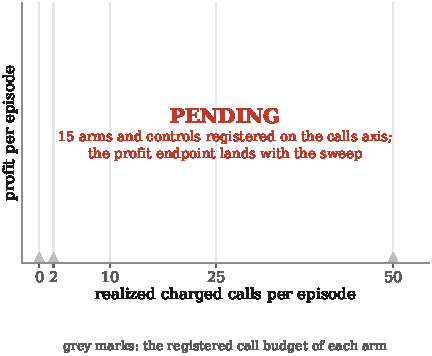
\includegraphics[width=\columnwidth]{fig3_frontier.pdf}
\caption{The frontier slot. Arms 8, 9 and 10 sit at the same horizontal position
by construction, because they share one physical proposal call set, so the
vertical spread among those three markers is exactly the effect of the
activation stage. The distance between the arm~1 floor and the oracle ceiling is
the only space any arm can win in, which makes this the headroom figure as well.
The calls axis is registered in advance and drawn; the profit endpoint is
\pending{reward against compute: one marked point per arm on realized charged
calls, with seed-level cluster-bootstrap intervals, the arm~1 floor, the oracle
ceiling and the non-dominated front}}
\label{fig:frontier}
\end{figure}

Efficiency is reported against the frontier of Fig.~\ref{fig:frontier} rather
than as a table of call counts, because the question is never how many calls an
arm made but how much profit those calls bought against the only headroom
available.
\pending{activation ablation, null-audit calibration and fragility, content
against timing, efficiency and frontiers, operational and hypothesis metrics,
traced cases}

\section{Related Work}
\label{sec:related}

Which ingredient is new? None. The handshake is.

\textbf{Language models for operations.} InventoryBench established the
complementarity this paper starts from, and its four strategies are our arms 1,
3, 5 and 11~\cite{inventorybench}. A design-time session can synthesize reusable
operations research algorithms outright~\cite{llm-or-algorithms}, and InvEvolve
evolves white-box inventory policies online~\cite{invevolve}. Our model does the
opposite of both: it estimates the environment rather than the policy, writes no
code, and every action stays fixed-form operations research. InvEvolve has no
public code artifact as of our search, so any comparison against it must be
labeled a faithful reimplementation, and we have not implemented one. Language
models reach the operations loop in other shapes as well: as a multi-agent
inventory manager~\cite{invagent}, as a reader of event text for demand
forecasting~\cite{eventcast}, and as a human-in-the-loop instruction channel
into a controller~\cite{instructmpc}; the same replenishment setting has a
multi-agent reinforcement-learning benchmark~\cite{mabim}, and text-game agent
evaluation has its own benchmark~\cite{textarena}. Field evidence supports the
interface shape: judgmental adjustment of a forecast input
raised profitability by 4.92 percent on average in a retail
experiment~\cite{kesavan-field}, and average United States import shipping delay
rose by 21 days between 2018 and 2024~\cite{carreras-valle-delays}.

\textbf{When to call, and what to commit to.} Event-triggered invocation with
threshold, CUSUM, sequential probability ratio~\cite{wald-sprt},
Bayesian~\cite{bocpd} and learned rules is already
established~\cite{event-triggered-llm}. Agents ask the same when-to-call
question of themselves, answered by gating over fast-slow planning~\cite{asscg},
budgeted replanning~\cite{brace} and learned model routing~\cite{routellm}, so
we treat invocation as fixed infrastructure and claim nothing about it. Structuring a plan as falsifiable commitments with confirming
and falsifying evidence, and running a hypothesis lifecycle with provenance and
belief updates, also exist already~\cite{fcpagent, hep}. What differs here is
that the commitment parameterizes an \emph{exogenous stochastic model} whose
influence is authorized by a preregistered sequential statistic and compiled into
inventory-control inputs, so the object is tested rather than merely recorded.

\textbf{Statistics and inventory theory.} We use e-values and anytime-valid
inference as given~\cite{vovk-wang-evalues, ramdas-savi, grunwald-safe-testing},
with the classical sequential and changepoint machinery behind them~\cite{ville,
wald-sprt, page-cusum, lorden, hinkley-changepoint}. The
nearest construction is the e-detector, which sums
processes started at every time and controls the average run
length~\cite{e-detectors}, while we start one only at model-selected stopping
times and control per-episode false activation by budget splitting. A theorem-backed
\emph{retirement} rule would need confidence sequences~\cite{howard-confseq},
specifically the forward and backward confidence-sequence intersection
test~\cite{shekhar-backward-cs}, which we do not adopt, which is why
our retirement rules are labeled empirical. The controller is the textbook
one~\cite{clark-scarf, zipkin-foundations}, with base-stock heuristics for
lost-sales systems, censored demand included, long
established~\cite{zipkin-lost-sales, huh-lost-sales}, and our transit-pause
semantics follow an established simulation convention in which material already
moving stops progressing~\cite{stockpyl}.

\section{Limitations}
\label{sec:limitations}

\textbf{One simulator, small pools.} All evidence comes from our generator. Outside the
noisy-lead stratum its lead times are deterministic, so a lead-time shift appears in the receipts
without noise, and that is where the gain sits: at $p/h = 4$ lead-time shifts, a sixth of the shocked episodes, carry
about 171 of the 178 per-episode gain over arm~1 with Gemini and 157 of 163 with Grok. With
noisy lead times the gain over arm~1 was not confirmed on eight units, and the one-period
shifts lost on average (descriptive). The method has not been run on InventoryBench's own instances, a third of
which have stochastic lead times with lost shipments; the fresh pools have 48 units (the confirmation
registered 72) because the alert bank yields distinct texts for only eight units per family.

\textbf{What the theorems cover.} Theorems~\ref{thm:exposure}
and~\ref{thm:regret} assume an exact null, and the arm as run lies outside it: its
demand null is estimated from the pre-proposal prefix, and its arrival null is a
diffuse delay law while our delays are deterministic outside the noisy-lead stratum.
A null Monte Carlo of the frozen arm (released with our code) finds no cell more
than two standard errors above a bound where the premise holds. With the plug-in
null and a first firing at period 10, in the cells matched to our null twins, it
measures $\Expect_0[\Pi_\sigma]$ at 2.0 to 2.7 times $A$ and
$\Prob_0(\sup_t \Pi_t \ge 1/2)$ at 2.3 to 3.7 times its bound (up to 3.2 and 4.7
in other cells); the arrival mismatch alone lifts exposure at a fixed decision to
at most 1.24 times its budget. The regret theorem bounds a one-period newsvendor
surrogate only.

\textbf{What the content-free control measures.} The control calls no model but
is timed by the same alerts, so it removes the text, not the alert channel. Its
null commitment also overstates action: a pulse hypothesis keeps its \eprocess{}
after its window closes, so its mass can linger on a null episode after it stops
moving the order. Post hoc, crediting each period's mass to its leading hypothesis,
pulse-led periods carry 0.69 of the control's 0.83 and 0.32 and 0.38 of the hedge's 0.52
and 0.46, so most of what the model's label removes is that mass.

\textbf{Status of the evidence.} Relative to Gate~3 this study is exploratory, and
Gate~3's decision, \emph{kill-or-reframe}, stands. The method was developed on the spent
pilot episodes; both later stages were registered, code frozen by hash, before their live
runs. The plan discloses a structural test on six first-stage units, an interim look at one
run, three departures from the original registration (net reward as endpoint, action before
any activation threshold, fresh units outside the frozen manifest), an audit that reproduced
every registered first-stage number, and the second stage's pre-run amendments, which changed
no hypothesis or cap (one clipped the noisy stratum's lead times). The second stage did not
establish null safety at $p/h = 19$, nor non-inferiority against arm~1 at $p/h = 1$ with Grok.

\section{Conclusion}
\label{sec:conclusion}

Asking a language model what changed, in a closed vocabulary, and testing the answer on later
data is a sound interface; letting the test switch the answer on is not enough: the registered
gate acted late or not at all, on whatever size the model stated. Certify-then-hedge keeps the
certificate and changes its use: the \eprocess{} prices hypotheses, the data size them, and the
controller hedges at the critical fractile of the resulting mixture. Under a known null and arrival law that
rule keeps the gate's error budget as a bound on expected exposure for any model output, and in
exploratory tests registered before their live runs it beat the gate at all three of the
benchmark's cost ratios and the operations research baseline at the middle and highest, with two
proposer models, though at the highest non-inferiority on no-shock episodes was not
established and on noisy lead times the gain over the baseline was not confirmed. On this
simulator the value came mostly from mechanisms the alert-timed content-free control shares,
concentrated in lead-time shifts; the text cut commitment on no-shock episodes and, when
stockouts dominate, added value with one of the two models. Whether text earns more where it
says what the data reveal only late, under a null the guarantee fully covers and on
InventoryBench's own stochastic lead times and lost shipments, is the question this design can
now answer.

% Sponsor acknowledgments belong in \thanks in the author block, not here.
% sections/13_acknowledgment.tex -- unnumbered, before the references.
% The preferred American spelling is "Acknowledgment" (no "e" after the "g").
% Sponsor acknowledgments belong in the unnumbered footnote on the first page
% (\thanks in the author block), not here.

\section*{Acknowledgment}

\pending{acknowledgments: funding, compute, and readers of the draft}


%%% --- References -------------------------------------------------------------------
% Only entries cited with \cite{...} appear in the References section.
% IEEEabrv.bib provides standard journal-name abbreviation strings for use
% inside entries in citations.bib; entry patterns for every type are in
% IEEEexample.bib.
\bibliographystyle{IEEEtran}
\bibliography{IEEEabrv,citations}

\end{document}
